\documentclass[11pt]{article}
\usepackage{amsmath,amsbsy,amssymb,verbatim,fullpage,ifthen,graphicx,bm,amsfonts,amsthm}
\usepackage{graphicx}
\usepackage{xcolor}
\newcommand{\mfile}[1]  {{\small \verbatiminput{./#1}}} % Jeff Fessler, input matlab file
\newcommand{\tmop}[1]{\ensuremath{\operatorname{#1}}}

\newcommand{\R}{\mathbb{R}}
\newcommand{\C}{\mathbb{C}}
\newcommand{\Z}{\mathbb{Z}}
\newcommand{\A}{\mathcal{A}}
\newcommand{\minimize}{\operatorname*{minimize\ }}
\newcommand{\maximize}{\operatorname*{maximize}}

%\newcommand{\mfile}[1]  {{\small \verbatiminput{./#1}}} 
\newcommand{\mtx}[1]{\mathbf{#1}}
\newcommand{\vct}[1]{\mathbf{#1}}
\def \lg       {\langle}
\def \rg       {\rangle}
\def \mA {\mtx{A}}
\def \mI {\mtx{I}}
\def \mU {\mtx{U}}
\def \mS {\mtx{S}}
\def \mV {\mtx{V}}
\def \mW {\mtx{W}}
\def \mLambda {\mtx{\Lambda}}
\def \mX {\mtx{X}}
\def \mY {\mtx{Y}}
\def \mZ {\mtx{Z}}
\def \zero     {\mathbf{0}}
\def \vzero    {\vct{0}}
\def \vone    {\vct{1}}
\def \vu {\vct{u}}
\def \vv {\vct{v}}
\def \vx {\vct{x}}
\def \vy {\vct{y}}
\def \vz {\vct{z}}
\def \vphi {\vct{\phi}}
\def \vmu {\vct{\mu}}
\def \R {\mathbb{R}}
\def \mepsilon {\mtx{\epsilon}}
\def \msigma {\mtx{\sigma}}
\def \mbeta {\mtx{\beta}}


\usepackage{xspace}

\makeatletter
\DeclareRobustCommand\onedot{\futurelet\@let@token\@onedot}
\def\@onedot{\ifx\@let@token.\else.\null\fi\xspace}

\def\eg{\emph{e.g}\onedot} \def\Eg{\emph{E.g}\onedot}
\def\ie{\emph{i.e}\onedot} \def\Ie{\emph{I.e}\onedot}
\def\cf{\emph{c.f}\onedot} \def\Cf{\emph{C.f}\onedot}
\def\etc{\emph{etc}\onedot} \def\vs{\emph{vs}\onedot}
\def\wrt{w.r.t\onedot} \def\dof{d.o.f\onedot}
\def\etal{\emph{et al}\onedot} \def\st{\emph{s.t}\onedot}
\pagestyle{plain}

\title{{\bf Homework Set 1, CPSC 8420, Spring 2022}}
\author{\Large\underline{Huang, Gangtong}}
\date{\textbf{\Large\textcolor{red}{Due 03/03/2022, Thursday, 11:59PM EST}}}

\begin{document}
\maketitle

\section*{Ridge Regression}
Please show that for arbitrary $\mA\in\R^{n\times p}$, $(\mA^T\mA+\lambda\mI_p)^{-1}\mA^T=\mA^T(\mA\mA^T+\lambda\mI_n)^{-1}$, where $\lambda>0$. Now assume $n=100$, please compare the time consumption when $p=[10,100,1000,2000]$ and plot the results appropriately (\eg in one figure where $X$-axis denotes $p$ while $Y$-axis the time consumption).
%For PCA, from the perspective of minimizing reconstruction error, please derive the solution to $\minimize \limits_{\bm{\mu},\{\vv_i\},\mU_q} \sum_{i=1}^{N}\|\mX_i-\bm{\mu}-\mU_q \vv_i\|^2_2, \st \ \mU_q^T\mU_q=\mI_q$, where $\mX\in\R^{p\times N}, \bm{\mu}\in\R^p, \mU \in\R^{p\times q}, \vv_i \in \R^q$. 
\\ \\
{\bf 1. Proof of $(\mA^T\mA+\lambda\mI_p)^{-1}\mA^T=\mA^T(\mA\mA^T+\lambda\mI_n)^{-1}$ }
\\ \\
$(\mA^T\mA+\lambda\mI_p)^{-1}\mA^T=\mA^T(\mA\mA^T+\lambda\mI_n)^{-1}\\=\mA^T\mA\mA^T+\lambda\mI_p\mA^T\\=\mA^T\mA\mA^T+\lambda\mA^T\\=\mA^T\mA\mA^T+\mA^T\lambda\\=   \mA^T(\mA\mA^T+\lambda)\\=\mA^T(\mA\mA^T+\lambda\mI_n)$
\\ \\
{\bf 2. Time consumption with varied $p$ }
\\ \\
Implemented with Python.
\\ 
\begin{figure}[h] % This is how figure are placed into latex document
\centering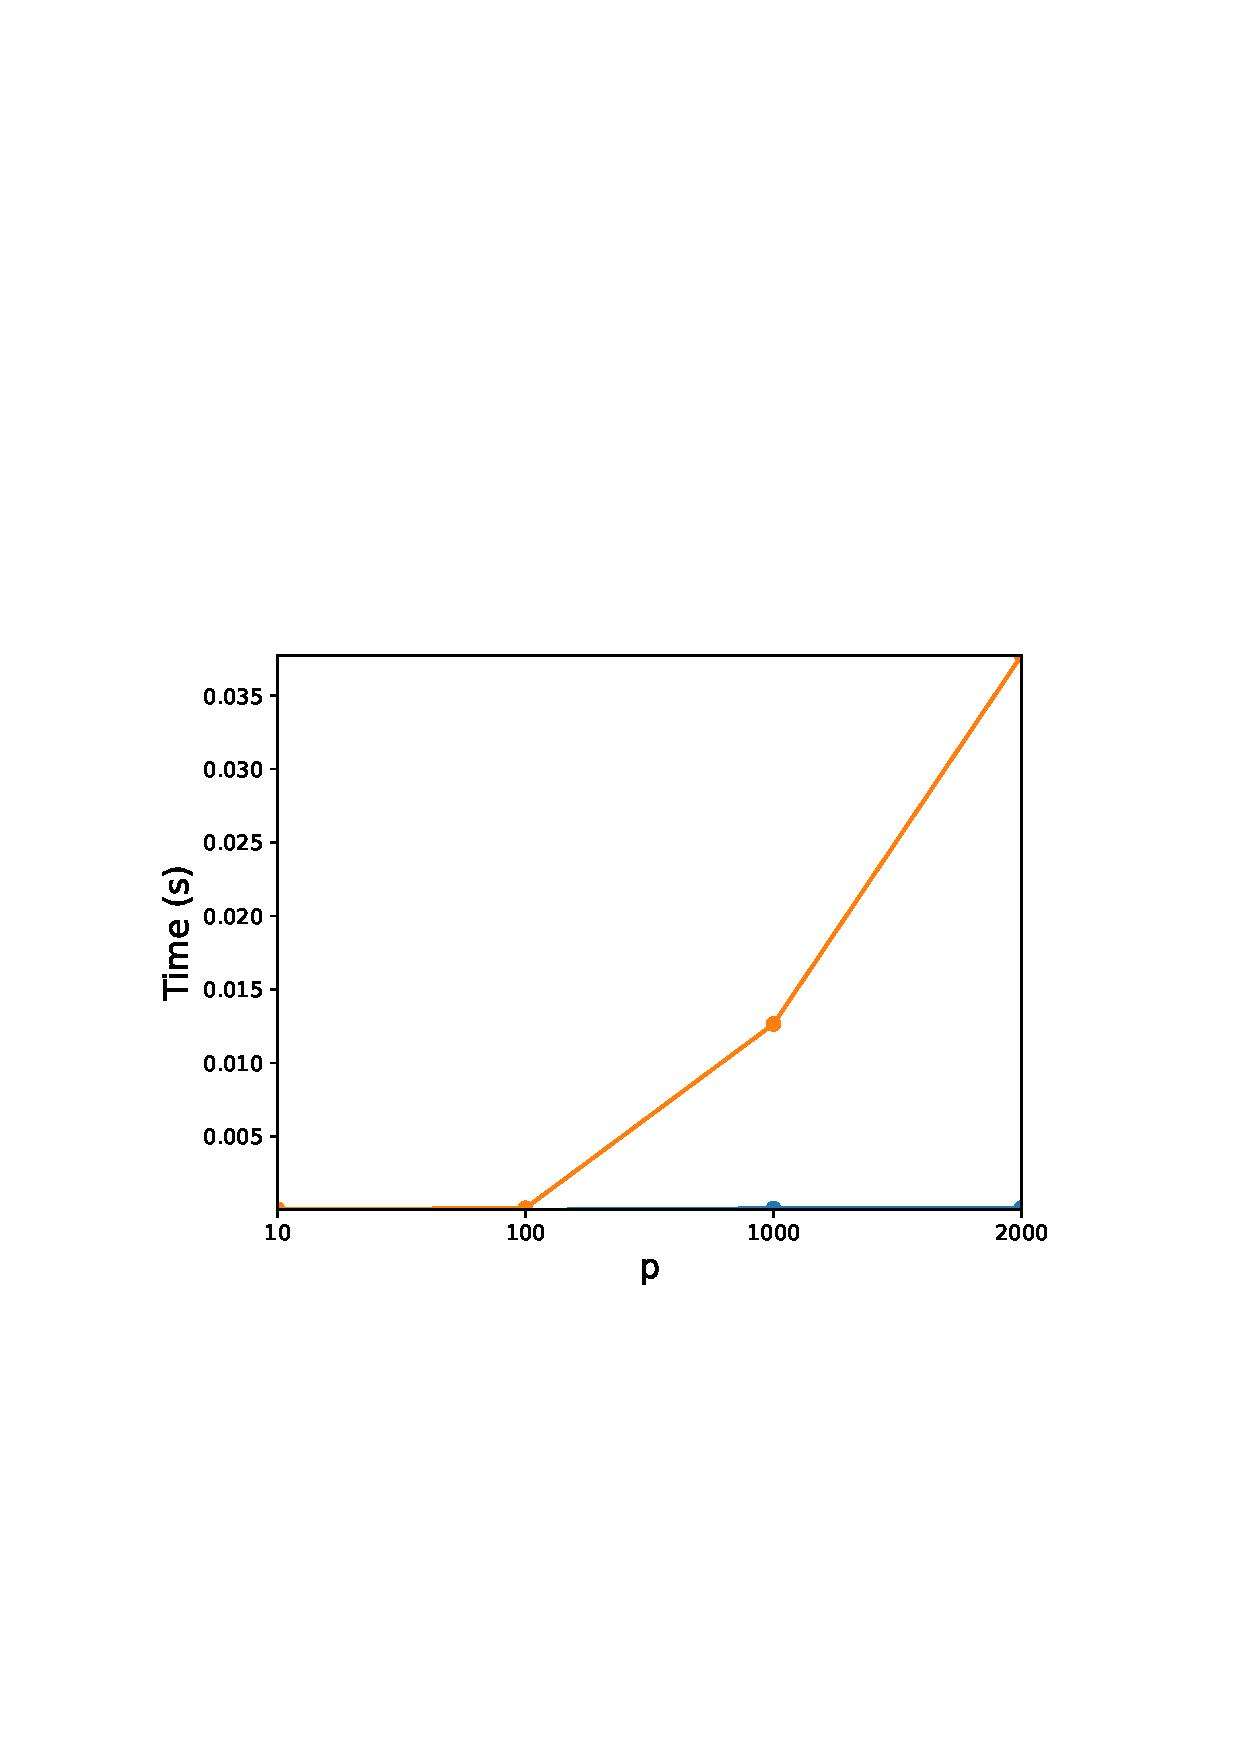
\includegraphics[width=0.45\linewidth]{prob1.png}
\caption{Ridge regression time consumption with varied $p$.} % caption of the figure
\label{fig:prob1}  % Label the figure so you can refer to it in text.
\end{figure}
\vspace{4cm}

\section*{Bias–variance trade-off for $k$-NN}
Assume $y=f(x)+\epsilon$ where $E(\epsilon)=0, Var(\epsilon)=\sigma^2$. Please show that:
\begin{equation}
	Err(x_0)=\sigma^2+\frac{\sigma^2}{k}+[f(x_0)-\frac{1}{k}\sum_{l=1}^{k}f(x_l)]^2,
\end{equation}
where $x_l$ denotes the nearest neighbour data.  Please justify Bias and Variance change when $k$ increases and explain if necessary.
%For PCA, from the perspective of maximizing variance, please show that the sotution of $\bm{\phi}$ to $\maximize \|\mX \bm{\phi}\|^2_2, \st \ \|\bm{\phi}\|_2=1$ is exactly the first column of $\mU$, where $[\mU,\mS,\mU]=svd(\mX^T\mX)$. (Note: you need prove why it is optimal than any other reasonable combinations of $\mU_i$, say $\hat{\bm{\phi}}=0.8*\mU(:,1)+0.6*\mU(:,2)$ which also  satisfies $\|\hat{\bm{\phi}}\|_2=1$.)
\\ \\
\begin{equation}
\begin{aligned}
Err(x_0) &= Err[(y-\hat{f}_k(x))^2 | x=x_0]\\
&=Err[(y-\hat{f}_k(x_0))^2]\\
&=Var(\hat{f}(x_0))+Bias(\hat{f}(x_0))^2+Var(\mepsilon)
\end{aligned}
\end{equation}
\\ \\
Denote the $l$-th neighbor of $x_0$'s nearest neighbor as $x_l$, then:  
\begin{equation}
\hat{f}(x_0) =\frac{1}{k}\sum_{l=1}^{k}y(x_l) =\frac{1}{k}\sum_{l=1}^{k}[f(x_l)+\mepsilon]
\end{equation}
\\ \\
\begin{equation}
\begin{aligned}
Var(\hat{f}(x_0)) &= Var\{\frac{1}{k}\sum_{l=1}^{k}[f(x_l)+\mepsilon]\}\\
&= \frac{1}{k^2}Var\{\sum_{l=1}^{k}[f(x_l)+\mepsilon]\}\\
&= \frac{1}{k^2}\sum_{l=1}^{k}Var(f(x_l)+\mepsilon)\\
&= \frac{1}{k^2}\sum_{l=1}^{k}\{Var[f(x_l)]+Var(\mepsilon_i)\}\\
\end{aligned}
\end{equation}
\\
And because $Var[f(x_l)]=0$, $Var(\mepsilon_i)=\msigma^2$, \\
\begin{equation}
	Var(\hat{f}(x_0)) = \frac{1}{k^2}k\msigma^2=\frac{\msigma}{k}
\end{equation}
\\ \\

\begin{equation}
\begin{aligned}
Bias(\hat{f}_k(x_0)) &= (y(x_0)-E(\hat{f}_k(x_0)))^2\\
&= [f{x_0}+\mepsilon-\frac{1}{k}\sum_{l=1}^{k}(y(x_l))]^2\\
&= [f{x_0}+\mepsilon-\frac{1}{k}\sum_{l=1}^{k}(f(x_l)+\mepsilon)]^2\\
&= [f{x_0}+\mepsilon-\frac{1}{k}\sum_{l=1}^{k}(f(x_l))-\frac{1}{k}k\mepsilon]^2\\
&= [f{x_0}-\frac{1}{k}\sum_{l=1}^kf(x_l)]^2\\
\end{aligned}
\end{equation}
Combining Equations (4)-(6), we have: 
\begin{equation}
\begin{aligned}
Err(x_0) &= Err[(y-\hat{f}_k(x))^2 | x=x_0]=Var(\hat{f}(x_0))+Bias(\hat{f}(x_0))^2+Var(\mepsilon)\\
&=\sigma^2+\frac{\sigma^2}{k}+[f(x_0)-\frac{1}{k}\sum_{l=1}^{k}f(x_l)]^2
\end{aligned}
\end{equation}


\section*{Shrinkage Methods}
For vanilla linear regression model: $\min \|\vy-\mA\bm{\beta}\|_2^2$, 
%where we set $\mA^T\mA=\mI$ for convinience, \frac{\lambda}{2}
we denote the solution as $\hat{\bm{\beta}}_{LS}$; for ridge regression model: $\min \|\vy-\mA\bm{\beta}\|_2^2+\lambda*\|\bm{\beta}\|_2^2$, we denote the solution as $\hat{\bm{\beta}}_\lambda^{Ridge}$; for Lasso model: $\min \frac{1}{2}\|\vy-\mA\bm{\beta}\|_2^2+\lambda*\|\bm{\beta}\|_1$, we denote the solution as $\hat{\bm{\beta}}_\lambda^{Lasso}$; for Subset Selection model:  $\min \frac{1}{2}\|\vy-\mA\bm{\beta}\|_2^2+\lambda*\|\bm{\beta}\|_0$, we denote the solution as $\hat{\bm{\beta}}_\lambda^{Subset}$, now please derive each $\hat{\bm{\beta}}$ given $\vy, \mA  (\st \ \mA^T\mA=\mI), \lambda$. Also, show the relationship of (each element in) $\hat{\bm{\beta}}_\lambda^{Ridge}, \hat{\bm{\beta}}_\lambda^{Lasso}, \hat{\bm{\beta}}_\lambda^{Subset}$ with (that in) $\hat{\bm{\beta}}_{LS}$ respectively. (you are encouraged to illustrate the relationship with figures appropriately.)
\vspace{4cm}

\section*{Linear Regression and its extension}
\begin{figure}
	\centering
	\includegraphics[width=1\linewidth]{fig}
	\caption{MSE vs (a) training set size, (b) polynomial degree, (c) size of ridge penalty. Solid Red = training, dotted black = test.}
	\label{fig:fig}
\end{figure}

In the Boston housing dataset, there are 506 records. We will
use first 13 features as inputs, $x$, and the 14th feature, median house price, as the output $y$. All features are continuous,
except feature 4, which is binary. However, we will treat this like any other continuous variable.
\begin{enumerate}
	\item Load the housing.data file. We will use the first 300 cases for training and the remaining 206 cases for
	testing. However, the records seem to be sorted in some kind of order. To eliminate this, we will shuffle the data
	before splitting into a training/test set. So we can all compare results, let use the following convention:
	\mfile{sample.m}


	\item Now extract the first n records of the training data, for $n \in \{25, 50, 75, 100, 150, 200, 300\}$. For each such
	training subset, standardize it (you may use \textit{zscore} function in Matlab), and fit a linear regression model using least squares. (Remember to include
	an offset term.) Then standardize the whole test set in the same way. Compute the mean squared error on
	the training subset and on the whole test set. Plot MSE versus training set size. You should get a plot like
	Figure 1(a). Turn in your plot and code. Explain why the test error decreases as n increases, and why the train
	error increases as n increases. Why do the curves eventually meet?
	As a debugging aid, here are the regression weights I get when I train on the first 25 cases (the first term is the
	offset, w0): $[26.11, -0.58, 3.02,\dots,-0.21, -0.27, -1.16]$.
\\ \\
The optimum parameter in linear regression is: $\hat{\mbeta}=(X^TX)^-1X^TY$. The linear regression is implemented with MatLAB (code in Appendix). The testing and training errors with varied training set size are shown in Fig. 3. See codes in Appendix.

\begin{figure}[h] % This is how figure are placed into latex document
\centering\includegraphics[width=0.45\linewidth]{prob4_2.png}
\caption{Ridge regression time consumption with varied $p$.} % caption of the figure
\label{fig:prob4_2}  % Label the figure so you can refer to it in text.
\end{figure}

The increase in training error is caused by the increased number of data points that is to fit with the linear model, while the decrease in the testing error is the result of the linear fit being more accurate due to larger training set size. \\
Since all the data points that constitute both the training and testing sets share the same source, it can be expected that the  random error per data point, $\mepsilon$, is similar across all data points, i.e. the variability of the data points is stable. The convergence between the testing and training data set occurs because the training and testing set sizes (300 and 206) are similar.
\\


	\item We will now replace the original features with an expanded set of features based on higher order terms. (We
	will ignore interaction terms.) For example, a quadratic expansion gives:
	\begin{equation}
		\begin{pmatrix}
			x_{11} & x_{12} & \dots & x_{1d} \\
			\vdots& \vdots & \ddots & \vdots \\
			x_{n1}& x_{n2} & \dots & x_{nd} \\
		\end{pmatrix}\xrightarrow[]{}\begin{pmatrix}
			x_{11} & x_{12} & \dots & x_{1d}& x_{11}^2 & x_{12}^2 & \dots & x_{1d}^2\\
			\vdots& \vdots & \ddots & \vdots&\vdots& \vdots & \ddots & \vdots \\
			x_{n1}& x_{n2} & \dots & x_{nd}& x_{n1}^2& x_{n2}^2 & \dots & x_{nd}^2\\
		\end{pmatrix}
	\end{equation}

The provided function degexpand(X,deg,addOnes) will replace each row of X with all powers up to degree deg. Use
this function to train (by least squares) models with degrees 1 to 6. Use all the the training data. Plot the MSE on
the training and test sets vs degree. You should get a plot like Figure 1(b). Turn in your plot and code. Explain
why the test error decreases and then increases with degree, and why the train error decreases with degree.
\\ \\

The optimum parameter in linear regression is: $\hat{\mbeta}=(X^TX)^-1X^TY$, where the training set $X$ is now expanded with quadratic terms. The testing and training errors with varied degrees of polynomials $deg$ are shown in Fig. 4. See codes in Appendix.

\begin{figure}[h] % This is how figure are placed into latex document
\centering\includegraphics[width=0.45\linewidth]{prob4_3.png}
\caption{Ridge regression time consumption with varied $p$.} % caption of the figure
\label{fig:prob4_3}  % Label the figure so you can refer to it in text.
\end{figure}

Degree expansion can increase the degrees of freedom of the fitting model and let the model approximate the data points with more flexibility. The training error monotonically decrease with increasing degrees of polynomial expansion, because with more parameters the fitting to the training set will improve. The testing error reaches a minimum at degree of expansion $deg=2$, indicating an improvement in the predictive performance of the model over the one without degree expansion. However, due to overfitting at higher $deg$ values, the testing error then increases with increasing $deg$ and reaches a peak at $deg=5$. \\ \textbf{Note:} the result presented in Fig. 4 saw a significant decrease as testing error as $deg$ increases from 5 to 6. As a reference, we can compare this result with the result in Fig. 5 at $\lambda=0$, since when $\lambda=0$, we have $\hat{\mbeta}_{linear}=(X^TX)^-1X^TY=(X^TX+0\mI_n)^{-1}X^TY=\hat{\mbeta}_{ridge}(\lambda=0)$, which are both $MSE_{test}\approx22$ and $MSE_{train}\approx10$. The identical results rule out the possibility of calculation errors. The rapid decrease in testing error may be due to other reasons. For example, testing error may actually reach a local minimum at $deg=6$, but then increase with larger $deg$. 
\\ \\

\item Now we will use ridge regression to regularize the degree 6 polynomial. Fit models using ridge regression with
the following values for $\lambda$:
$$lambdas=[0 \  logspace(-10,10,10)]$$
Use all the training data. Plot the MSE on the training and test sets vs $log_{10}(\lambda)$. You should get a plot like
Figure 1(c). Turn in your plot and code. Explain why the test error goes down and then up with increasing $\lambda$,
and why the train error goes up with increasing $\lambda$.
\\ \\
The optimum parameter in ridge regression is: $\hat{\mbeta}=(X^TX+\lambda\mI_n)^{-1}X^TY$. The testing and training errors with varied $\lambda$ are shown in Fig. 5. See codes in Appendix.

\begin{figure}[h] % This is how figure are placed into latex document
\centering\includegraphics[width=0.45\linewidth]{prob4_4.png}
\caption{Ridge regression time consumption with varied $p$.} % caption of the figure
\label{fig:prob4_4}  % Label the figure so you can refer to it in text.
\end{figure}

The penalty term in ridge regression, $\lambda$, imposes constraints on the magnitudes of elements in $\hat{\mbeta}$ to avoid overfitting. Since $\hat{\mbeta}_{linear}=(X^TX)^{-1}X^TY$ already gives the optimal linear fit to the training data set, the deviation of $\hat{\mbeta}_{ridge}$ from $\hat{\mbeta}_{linear}$ caused by $\lambda$ will result in the increase of $MSE_{train}$. The constraints on magnetudes of parameters avoids overfitting and can improve the predictive performance of the fitting model, as reflected in Fig. 5 when $log(\lambda)$ increases from -10 to 1. However, larger penalty term will supress the contribution of certain parameters to the fitting model, which may cause the loss of information represented by these parameters and eventually affect the accuracy of the fitting model.

\item We turn to Lasso method with objective $\frac{1}{2}\|\mX \beta-y\|^2+\lambda\|\beta\|_1$ where $\lambda$ varies in: $lambdas=[logspace(-10,10,10)]$ and we make use of all training samples with no feature expansion. Please plot the changes of $\beta$ with $\lambda$ changes.

The optimum parameter in Lasso method does not have an analytical solution and can only be solved numerically. The testing and training errors with varied $\lambda$ are shown in Fig. 5. See codes in Appendix.
\\ \\
\begin{figure}[h] % This is how figure are placed into latex document
\centering\includegraphics[width=0.75\linewidth]{prob4_5.png}
\caption{Ridge regression time consumption with varied $p$.} % caption of the figure
\label{fig:prob4_5}  % Label the figure so you can refer to it in text.
\end{figure}

As expected, the Lasso method supresses the magnitudes of parameters. With larger $\lambda$ the parameters effectively approximate 0.

\end{enumerate}

\section*{Appendix}

\textbf{Problem 4.2: Linear regression implemented with MatLab}\\
\begin{verbatim}
clear all;

data = load('housing.data');
x = data(:, 1:13);
y = data(:, 14);
[n,d] = size(x);
seed = 2; rand('state',seed); randn('state', seed);
perm = randperm(n); % remove any possible ordering fx
x = x(perm,:); y = y(perm);
N = length(data);

l_mseTrain = [];
l_mseTest = [];

for Ntrain = [25 50 75 100 150 200 300]
    Ntest = N - Ntrain;

    Xtrain = x(1:Ntrain,:); ytrain = y(1:Ntrain);
    %Standardization
    Xtraincent = zscore(Xtrain); 
    Xtest = x(Ntrain+1:end,:); ytest = y(Ntrain+1:end);
    Xtestcent = zscore(Xtest);

    XtrainApp = [ones(Ntrain,1) Xtraincent];
    XtestApp = [ones(Ntest,1) Xtestcent];

    beta_hat = pinv(XtrainApp'*XtrainApp)*XtrainApp'*ytrain;

    ytrainPred = beta_hat' * XtrainApp';
    ytestPred = beta_hat' * XtestApp';

    seTrain = 0;
    for i = 1:Ntrain
        seTrain = (ytrainPred(i) - ytrain(i))^2 + seTrain;
    end
    mseTrain = seTrain/Ntrain;
    l_mseTrain = [l_mseTrain, mseTrain];

    seTest = 0;
    for i = 1:Ntest
        seTest = (ytestPred(i) - ytest(i))^2 + seTest;
    end
    mseTest = seTest/Ntest;
    l_mseTest = [l_mseTest, mseTest];
end

% Plotting
hold on
scatter([25 50 75 100 150 200 300],l_mseTrain,'red','filled')
line([25 50 75 100 150 200 300],l_mseTrain,'Color','red')
xlabel("Training set size")
%xticks([1:7])
%xticklabels([25 50 75 100 150 200 300])
ylabel("MSE")
scatter([25 50 75 100 150 200 300],l_mseTest,'blue','filled')
line([25 50 75 100 150 200 300],l_mseTest,'Color','blue')
legend('Training','','Test','')
\end{verbatim}

\textbf{Problem 4.3: Degree expansion and linear regression implemented with MatLab}\\

\begin{verbatim}
clear all;

data = load('housing.data');
x = data(:, 1:13);
y = data(:, 14);
[n,d] = size(x);
seed = 2; rand('state',seed); randn('state', seed);
perm = randperm(n); % remove any possible ordering fx
x = x(perm,:); y = y(perm);
N = length(data)

Ntrain = 300;
Ntest = N - Ntrain;
Xtrain = x(1:Ntrain,:); ytrain = y(1:Ntrain);
Xtest = x(Ntrain+1:end,:); ytest = y(Ntrain+1:end);
Xtraincent = zscore(Xtrain);
Xtestcent = zscore(Xtest);


l_mseTrain = [];
l_mseTest = [];

%Standardize twice

for deg = [1 2 3 4 5 6]
    %Standardize and add the constant column
    XtrainApp = degexpand(Xtraincent,deg,1);
    XtestApp = degexpand(Xtestcent,deg,1);

    beta_hat = pinv(XtrainApp'*XtrainApp)*XtrainApp'*ytrain;

    ytrainPred = beta_hat' * XtrainApp';
    ytestPred = beta_hat' * XtestApp';

    seTrain = 0;
    for i = 1:Ntrain
        seTrain = (ytrainPred(i) - ytrain(i))^2 + seTrain;
    end
    mseTrain = seTrain/Ntrain;
    l_mseTrain = [l_mseTrain, mseTrain];
    
    seTest = 0;
    for i = 1:Ntest
        seTest = (ytestPred(i) - ytest(i))^2 + seTest;
    end
    mseTest = seTest/Ntest;
    l_mseTest = [l_mseTest, mseTest];

end
l_mseTest
l_mseTrain

%% Plotting %%
hold on
N_pts = 6
scatter([1:N_pts],l_mseTrain,'red','filled')
line([1:N_pts],l_mseTrain,'Color','red')
xlabel("Degree of expansion")

ylabel("MSE")
scatter([1:N_pts],l_mseTest,'blue','filled')
line([1:N_pts],l_mseTest,'Color','blue')
legend('Training','','Test','')
%% Function definitions %%
function xx = degexpand(x, deg, addOnes)
    % Expand input vectors to contain powers of the input features
    % This file is from pmtk3.googlecode.com
    
    [n,m] = size(x);
    if nargin < 3
        addOnes = 0; 
    end
    
    xx = repmat(x, [1 1 deg]);
    degs = repmat(reshape(1:deg, [1 1 deg]), [n m]);
    xx = xx .^ degs;
    xx = reshape(xx, [n, m*deg]);
    
    if addOnes
      xx = [ones(n,1) xx];
    end
end
\end{verbatim}

\textbf{Problem 4.4: Degree expansion and ridge regression implemented with MatLab}\\

\begin{verbatim}
clear all;

data = load('housing.data');
x = data(:, 1:13);
y = data(:, 14);
[n,d] = size(x);
seed = 2; rand('state',seed); randn('state', seed);
perm = randperm(n); % remove any possible ordering fx
x = x(perm,:); y = y(perm);
N = length(data)

Ntrain = 300;
Ntest = N - Ntrain;
Xtrain = x(1:Ntrain,:); ytrain = y(1:Ntrain);
Xtest = x(Ntrain+1:end,:); ytest = y(Ntrain+1:end);
Xtraincent = zscore(Xtrain);
Xtestcent = zscore(Xtest);

l_mseTrain = [];
l_mseTest = [];

lambdas = [0 logspace(-10, 10, 10)]

for lambda = lambdas
    Ntest = N - Ntrain;

    Xtrain = x(1:Ntrain,:); ytrain = y(1:Ntrain);
    %Standardization
    Xtraincent = zscore(Xtrain); 
    Xtest = x(Ntrain+1:end,:); ytest = y(Ntrain+1:end);

    XtrainApp = degexpand(Xtraincent,6,1);
    XtestApp = degexpand(Xtestcent,6,1);
    
    beta_hat = pinv(XtrainApp'*XtrainApp + lambda*eye(79))*XtrainApp'*ytrain;

    ytrainPred = beta_hat' * XtrainApp'
    ytestPred = beta_hat' * XtestApp'

    seTrain = 0;
    for i = 1:Ntrain
        seTrain = (ytrainPred(i) - ytrain(i))^2 + seTrain;
    end
    mseTrain = seTrain/Ntrain;
    l_mseTrain = [l_mseTrain, mseTrain];
    
    seTest = 0;
    for i = 1:Ntest
        seTest = (ytestPred(i) - ytest(i))^2 + seTest;
    end
    mseTest = seTest/Ntest;
    l_mseTest = [l_mseTest, mseTest];
end

l_mseTest
l_mseTrain

%% Plotting
hold off
hold on
lambdas_plt = arrayfun(@(x) log10(x), lambdas)
scatter(lambdas_plt,l_mseTrain,'red','filled')
line(lambdas_plt,l_mseTrain,'Color','red')
xlabel("log(lambda)")
ylabel("MSE")
scatter(lambdas_plt,l_mseTest,'blue','filled')
line(lambdas_plt,l_mseTest,'Color','blue')
legend('Training','','Test','')

%% Reference using built-in ridge() function
% 
% l_mseTrain = [];
% l_mseTest = [];
% 
% for lambda = lambdas
%     B = ridge(ytrain, XtrainApp, lambda)
%     ytrainPred = B' * XtrainApp'
%     ytestPred = B' * XtestApp'
% 
%     seTrain = 0;
%     for i = 1:Ntrain
%         seTrain = (ytrainPred(i) - ytrain(i))^2 + seTrain;
%     end
%     mseTrain = seTrain/Ntrain;
%     l_mseTrain = [l_mseTrain, mseTrain];
%     
%     seTest = 0;
%     for i = 1:Ntest
%         seTest = (ytestPred(i) - ytest(i))^2 + seTest;
%     end
%     mseTest = seTest/Ntest;
%     l_mseTest = [l_mseTest, mseTest];
% end
% 
% hold off
% hold on
% lambdas_plt = arrayfun(@ (x) log(x), lambdas)
% scatter(lambdas_plt,l_mseTrain,'red','filled')
% line(lambdas_plt,l_mseTrain,'Color','red')
% xlabel("Training set size")
% %xticks([1:7])
% %xticklabels([25 50 75 100 150 200 300])
% ylabel("MSE")
% scatter(lambdas_plt,l_mseTest,'blue','filled')
% line(lambdas_plt,l_mseTest,'Color','blue')
% legend('Training','','Test','')

%% 
function xx = degexpand(x, deg, addOnes)
    % Expand input vectors to contain powers of the input features
    % This file is from pmtk3.googlecode.com
    
    [n,m] = size(x);
    if nargin < 3
        addOnes = 0; 
    end
    
    xx = repmat(x, [1 1 deg]);
    degs = repmat(reshape(1:deg, [1 1 deg]), [n m]);
    xx = xx .^ degs;
    xx = reshape(xx, [n, m*deg]);
    
    if addOnes
      xx = [ones(n,1) xx];
    end
end
\end{verbatim}

\textbf{Problem 4.5: Lasso method implemented with MatLab}\\

\begin{verbatim}
clear all;

data = load('housing.data');
x = data(:, 1:13);
y = data(:, 14);
[n,d] = size(x);
seed = 2; rand('state',seed); randn('state', seed);
perm = randperm(n); % remove any possible ordering fx
x = x(perm,:); y = y(perm);
N = length(data)

Ntrain = 300;
Ntest = N - Ntrain;
Xtrain = x(1:Ntrain,:); ytrain = y(1:Ntrain);
Xtest = x(Ntrain+1:end,:); ytest = y(Ntrain+1:end);
Xtraincent = zscore(Xtrain);
Xtestcent = zscore(Xtest);

l_beta = [];

lambdas = [logspace(0,4)];

for lambda = lambdas
    beta_test = lassoAlg(Xtraincent, ytrain, lambda);  
    l_beta = [l_beta beta_test];
end

%Plotting
for i = length(l_beta)
    lambdas_plt = arrayfun(@(x) log10(x), lambdas);
    for i = [1 : length(l_beta(:,1))]
        plot(lambdas_plt,l_beta(i,:),'-*')
        hold on
    end
end
colormap(jet(13))
xlabel("log(lambda)")
ylabel("beta")
legends = arrayfun(@(x) strcat('beta',string(x)), [1:13])
legend('Parameters', legends)
%
% l_beta(1,:)

%% Lasso Optimization Algorithm %%
% inputs: A (nxd matrix), y (nx1 vector), lam (scalar)
% return: xh (dx1 vector)

function xh = lassoAlg(A,y,lam)     
    xnew = rand(size(A,2),1);   % "initial guess" 
    xold = xnew+ones(size(xnew)); % used zeros so the while loop initiates
    loss = xnew - xold;
    thresh = 10e-3;     % threshold value for optimization

    while norm(loss) > thresh
        xold = xnew;    % need to store the previous iteration of xh
        for i = 1:length(xnew)
            a = A(:,i);     % get column of A
            p = (norm(a,2))^2;
            % from notes: -t = sum(aj*xj) - y for all j != i
            % i.e., sum(aj*xj) - ai*xi - y (my interpretation)
            % hence t = (above) * -1
            % want to be sure this the correct definition of t?
            t =  a*xnew(i) + y - A*xnew; 
            q = a'*t;
            % update xi
            xnew(i) = (1/p) * sign(q) * max(abs(q)-lam, 0);
        end
        loss = xnew - xold;     % update loss 
    end
    xh = xnew;
end
\end{verbatim}

\end{document}
